\documentclass{article}
\usepackage{tikz}
\usetikzlibrary{positioning}

\tikzstyle{startstop} = [rectangle, rounded corners, minimum width=3cm, minimum height=1cm,text centered, draw=black, fill=red!30]
\tikzstyle{process} = [rectangle, minimum width=3cm, minimum height=1cm, text centered, draw=black, fill=blue!30]
\tikzstyle{file} = [rectangle, minimum width=3cm, minimum height=1cm, text centered, draw=black, fill=gray!30]
\tikzstyle{arrow} = [thick,->,>=stealth]    

\title{Project presentation}
\author{Pierre Bouvet}
\date{\today}

\begin{document}

\maketitle


\section{Introduction}
This document is made as to present the vision of the HDF\_BLS library and the software approach for the unification of all BLS data. This file is meant to be evolutive with the different needs encountered by researchers. It however presents succintly the current vision of the project and allows to better understand its development and its parts.

\section{HDF5 file structure}

    \subsection{Basic file structure}
        The vision of the project is to unify all BLS data into a single HDF5 file. This file will be used to store all the data and metadata of the BLS. The data will be stored in a hierarchical structure, all the data related to BLS being stored the "Data" group. This choice allows results from other techinques to be stored in the same file, only in other, independent groups, to minimize the risk of nomenclature competition between techinques. The "Data" group will contain all the data. These data are arranged in groups, whose identifiers are "Data\_i". Each group can only contain one measure, in the form of an array, whose dimension is however not restricted. This measure will be called "Raw\_data". The attributes of the measure are stored in the group attributes.

        The following structure represents the base structure of the file:

        \begin{verbatim}
            file.h5
            +-- Data (group)
            |   +-- Data_1 (group)
            |   |   +-- Raw_data (dataset)
        \end{verbatim}

    \subsection{Attributes}

        The attributes will follow a hierarchical structure. The attributes that apply to all "Data\_i" will be stored in the "Data" group, while the parameters that apply to a specific "Data\_i" will be stored in the "Data\_i" group. All the attributes are stored as text. Attributes are then divided in four categories:
        \begin{itemize}
            \item Attributes that are specific to the spectrometer used, such as the wavelength of the laser, the type of laser, the type of detector, etc. These attributes are recognized by the capital letter word "SPECTROMETER" in the name of the attribute.
            \item Attributes that are specific to the sample, such as the date of the measurement, the name of the sample, etc. These attributes are recognized by the capital letter word "MEASURE" in the name of the attribute.
            \item Attributes that are specific to the original file format, such as the name of the file, the date of the file, the version of the file, the precision used on the storage of the data, etc. These attributes are recognized by the capital letter word "FILEPROP" in the name of the attribute.
            \item Attributes that are used inside the HDF5 file, such as the name of the group, the name of the dataset, etc. These attributes are the only ones without a prefix.
        \end{itemize}

        The name of the attribues contains the unit of the attribute if it has units, in the shape of an underscore followed by the unit in parenthesis. Some parameters that can be represented by a series of norms will also be defined in a given norm, such as the ISO8601 for the date. These norms are however not specified in the name of the attribute. Here are some examples of attributes:
        \begin{itemize}
            \item "SPECTROMETER.Detector\_Type" is the type of the detector used.
            \item "MEASURE.Sample" is the name of the sample.
            \item "MEASURE.Exposure\_(s)" is the exposire of the sample given in seconds
            \item "MEASURE.Date\_of\_measurement" is the date of the measurement. 
            \item "FILEPROP.Name" is the name of the file.
        \end{itemize}

        To unify the name of attributes, a spreadsheet is accesible, containing all the attributes and their units. This spreadsheet will be updated as new attributes are added to the project and defined with a version number that will also be stored in the attribtutes of each data attributes (under FILEPROP.version). This spreadsheet is meant to be exported in a CSV file that can be used to update the attributes of the data.

    \subsection{Meta-files}
        It can be useful to store in a same file, measures coming from different instruments, taken in different conditions, or that we just want to separate from other groups of measures. In that end, we propose a tree-like structure of the HDF5 file, where each group can contain sub-groups, which can also contain sub-groups etc. In order to unify the way we access these groups, we propose to identify them by a unique identifier of the form "Data\_i", where "i" is an integer. Here is an example of the structure of a meta-file:

        \begin{verbatim}
            file.h5
            +-- Data
            |   +-- Data_1
            |   |   +-- Data_1
            |   |   |   +-- ...
            |   |   +-- Data_2
            |   |   |   +-- ...
            |   |   +-- ...
            |   +-- Data_2
            |   |   +-- Data_1
            |   |   |   +-- Data_1
            |   |   |   |   +-- ...
            |   |   |   +-- Data_2
            |   |   |   |   +-- ...
            |   |   |   ...
            |   |   ...
            |   ...
        \end{verbatim}

    \subsection{Complete structure definition}
        The file is intended to be used to store not only raw data but also treated data together with the parameters used for treatment. As such, we propose to complete the structure defined above with the following structure:

        \begin{verbatim}
            file.h5
            +-- Data (group)
            |   +-- Data_0 (group)
            |   |   +-- Raw_data (dataset)
            |   |   +-- Abscissa_0 (dataset)
            |   |   +-- Abscissa_1 (dataset)
            |   |   +-- ...
            |   |   +-- PSD (dataset)
            |   |   +-- Frequency (dataset)
            |   |   +-- Treat_0(group)
            |   |   |   +-- Shift (dataset)
            |   |   |   +-- Shift_std (dataset)
            |   |   |   +-- Linewidth (dataset)
            |   |   |   +-- Linewidth_std (dataset)
            |   |   +-- Treat_1(group)
            |   |   ...
            |   +-- Data_1 (group)
            |   ...
        \end{verbatim}

        The nomenclature is defined as follows:
        \begin{itemize}
            \item \textbf{"Data\_i"} is the identifier of the group containing the i-th measure.
            \item \textbf{"Raw\_data"} is the identifier of the dataset containing the raw data of the measure stored in the "Data\_i" group.
            \item \textbf{"Abscissa\_i"} is the identifier of the dataset containing the i-th abscissa array of "Raw\_data" and "PSD". The dimension of this dataset is not forced to one.
            \item \textbf{"PSD"} is the identifier of the dataset of the Power Spectrum Density of the measure, associated with the "Frequency" dataset. "Raw\_data" and "PSD" are arrays of same shape. We impose the last dimension(s) of "PSD" to be the same as the dimension(s) of "Frequency".
            \item \textbf{"Frequency"} is the identifier of the dataset containing the frequency axis of the "PSD".
            \item \textbf{"Treat\_i"} is the identifier of the group containing the treated data of the i-th measure.
            \item \textbf{"Shift"} is the identifier of the dataset containing the values of the fitted frequency shifts.
            \item \textbf{"Shift\_std"} is the identifier of the dataset containing the standard deviation of the fitted frequency shifts.
            \item \textbf{"Linewidth"} is the identifier of the dataset containing the values of the fitted linewidths.
            \item \textbf{"Linewidth\_std"} is the identifier of the dataset containing the standard deviation of the fitted linewidths.  
        \end{itemize}
        
    \subsection{Examples}
        
        \subsubsection{Example 1 - A single measure with no treatment}
            In this first example, we want to store a single measure of a water sample.
        
            The following structure represents the base structure of the file:
            \begin{verbatim}
                file.h5
                +-- Data (group) -> Name = "Measure"
                |   +-- Data_0 (group) -> Name = "Water"
                |   |   +-- Raw_data (dataset)
            \end{verbatim}
            Note that we have here added arrows and an example of the value of the "Name" attributes.
        
        \subsubsection{Example 2 - A series of measures with no treatment}
            In this second example, we want to store a series of measures taken on three different samples: Water, Ethanol and Glycerol.

            The following structure represents the base structure of the file:
            \begin{verbatim}
                file.h5
                +-- Data (group) -> Name = "Measure"
                |   +-- Data_0 (group) -> Name = "Water"
                |   |   +-- Raw_data (dataset)
                |   +-- Data_1 (group) -> Name = "Ethanol"
                |   |   +-- Raw_data (dataset)
                |   +-- Data_2 (group) -> Name = "Glycerol"
                |   |   +-- Raw_data (dataset)
            \end{verbatim}
            Note that we have here added arrows and an example of the value of the "Name" attributes.
        
        \subsubsection{Example 3 - A series of series of measures with no treatment but with a calibration spectrum and an impulse response measure}
            In this third example, we want to store a series of two measures taken on two different samples: Water and Ethanol. We also want to store a calibration curve and an impulse response curve.

            The following structure represents the base structure of the file:
            \begin{verbatim}
                file.h5
                +-- Data (group) -> Name = "Measure"
                |   +-- Data_0 (group) -> Name = "Impulse_Response"
                |   |   +-- Raw_data (dataset)
                |   +-- Data_1 (group) -> Name = "Calibration"
                |   |   +-- Raw_data (dataset)
                |   +-- Data_2 (group) -> Name = "Water"
                |   |   +-- Data_0 (group) -> Name = "Water_01"
                |   |   |   +-- Raw_data (dataset)
                |   |   +-- Data_1 (group) -> Name = "Water_02"
                |   |   |   +-- Raw_data (dataset)
                |   +-- Data_3 (group) -> Name = "Ethanol"
                |   |   +-- Data_0 (group) -> Name = "Ethanol_01"
                |   |   |   +-- Raw_data (dataset)
                |   |   +-- Data_1 (group) -> Name = "Ethanol_02"
                |   |   |   +-- Raw_data (dataset)
            \end{verbatim}
            Note that we have here added arrows and an example of the value of the "Name" attributes.
        
        \subsubsection{Example 4 - A single measure converted to a Power Spectrum Density}
            In this fourth example, we want to store a single measure of a water sample. This measure has been converted into a Power Spectrum Density.

            The following structure represents the base structure of the file:
            \begin{verbatim}
                file.h5
                +-- Data (group) -> Name = "Measure"
                |   +-- Data_0 (group) -> Name = "Water"
                |   |   +-- Raw_data (dataset)
                |   |   +-- PSD (dataset)
                |   |   +-- Frequency (dataset)
            \end{verbatim}
            Note that we have here added arrows and an example of the value of the "Name" attributes.
            In this case, all the steps of the conversion to PSD are stored in the "Data\_0" group. The nomenclature of the attribute(s) used to store the parameters of the treatment is not specified.
        
        \subsubsection{Example 5 - Multiple measures converted to a Power Spectrum Density with a time-independent spectrometer}
            In this fifth example, we are in the situation where a time-independent spectrometer has been used to acquire multiple measures. In this case, the hierrarchy of the file can be used to reduce the number of datasets, by considering that all the PSD share the same frequency axis.

            The following structure represents the base structure of the file:
            \begin{verbatim}
                file.h5
                +-- Data (group) -> Name = "Measure"
                |   +-- Frequency (dataset)
                |   +-- Data_0 (group) -> Name = "Sample_1"
                |   |   +-- Raw_data (dataset)
                |   |   +-- PSD (dataset)
                |   +-- Data_1 (group) -> Name = "Sample_2"
                |   |   +-- Raw_data (dataset)
                |   |   +-- PSD (dataset)
            \end{verbatim}
            Note that we have here added arrows and an example of the value of the "Name" attributes.

        \subsubsection{Example 6 - A single measure with a treatment}
            In this sixth example, we want to store a single measure of a water sample that has been treated.

            The following structure represents the base structure of the file:
            \begin{verbatim}
                file.h5
                +-- Data (group) -> Name = "Measure"
                |   +-- Data_0 (group) -> Name = "Water"
                |   |   +-- Raw_data (dataset)
                |   |   +-- PSD (dataset)
                |   |   +-- Frequency (dataset)
                |   |   +-- Treat_0 (group) -> Name = "Treat_5GHz"
                |   |   |   +-- Shift (dataset)
                |   |   |   +-- Shift_std (dataset)
                |   |   |   +-- Linewidth (dataset)
                |   |   |   +-- Linewidth_std (dataset)
            \end{verbatim}
            Note that we have here added arrows and an example of the value of the "Name" attributes.
            In this case, all the steps of the treatment are stored in the "Treat\_0" group. The nomenclature of the attribute(s) used to store the parameters of the treatment is not specified.
        
        \subsubsection{Example 7 - A single measure with two distinct treatments}
            In this seventh example, we will store a single measure where two different treatments have been performed (for example a measure at an interface between two materials).

            The following structure represents the base structure of the file:
            \begin{verbatim}
                file.h5
                +-- Data (group) -> Name = "Measure"
                |   +-- Data_0 (group) -> Name = "Water"
                |   |   +-- Raw_data (dataset)
                |   |   +-- PSD (dataset)
                |   |   +-- Frequency (dataset)
                |   |   +-- Treat_0 (group) -> Name = "Treat_5GHz"
                |   |   |   +-- Shift (dataset)
                |   |   |   +-- Shift_std (dataset)
                |   |   |   +-- Linewidth (dataset)
                |   |   |   +-- Linewidth_std (dataset)
                |   |   +-- Treat_1 (group) -> Name = "Treat_10GHz"
                |   |   |   +-- Shift (dataset)
                |   |   |   +-- Shift_std (dataset)
                |   |   |   +-- Linewidth (dataset)
                |   |   |   +-- Linewidth_std (dataset)
            \end{verbatim}
            Note that we have here added arrows and an example of the value of the "Name" attributes.
            In this case, all the steps of the treatment around 5GHz are stored in the "Treat\_0" group and the ones around 10GHz in the "Treat\_1" group. The nomenclature of the attribute(s) used to store the parameters of the treatment is not specified.

        \subsubsection{Example 8 - A single mapping stored as a single measure}
            In this eighth example, we want to store a mapping of a sample. This mapping has been obtained with a spectrometer that returns an array of points for all the points mapped. To clarify this example, we will indicate the dimension of each dataset here between brackets.

            The following structure represents the base structure of the file:
            \begin{verbatim}
                file.h5
                +-- Data (group) -> Name = "Measure"
                |   +-- Data_0 (group) -> Name = "Sample"
                |   |   +-- Raw_data (dataset) [X, Y, M]
                |   |   +-- PSD (dataset) [X, Y, N]
                |   |   +-- Frequency (dataset) [N]
                |   |   +-- Abscissa_0 (dataset) [X] -> Name = "x (mm)"
                |   |   +-- Abscissa_1 (dataset) [Y] -> Name = "y (mm)"
                |   |   +-- Treat_1 (group) -> Name = "Treat"
                |   |   |   +-- Shift (dataset) [X, Y]
                |   |   |   +-- Shift_std (dataset) [X, Y]
                |   |   |   +-- Linewidth (dataset) [X, Y]
                |   |   |   +-- Linewidth_std (dataset) [X, Y]
            \end{verbatim}
            Note that we have here added arrows and an example of the value of the "Name" attributes.
        
        \subsubsection{Example 9 - A series of mapping over the same field of view stored as a single measure}
            In this ninth example, we are in the situation where multiple mappings of same dimension have been obtained with a spectrometer that returns an array of points for all the points mapped. In this case, the hierrarchy of the file can be used to reduce the number of datasets, by considering that all the PSD share the same frequency axis and the same field of view.

            The following structure represents the base structure of the file:
            \begin{verbatim}
                file.h5
                +-- Data (group) -> Name = "Measure"
                |   +-- Abscissa_0 (dataset) [X] -> Name = "x (mm)"
                |   +-- Abscissa_1 (dataset) [Y] -> Name = "y (mm)"
                |   +-- Frequency (dataset) [N]
                |   +-- Data_0 (group) -> Name = "Day_1"
                |   |   +-- Raw_data (dataset) [X, Y, M]
                |   |   +-- PSD (dataset) [X, Y, N]
                |   |   +-- Treat_1 (group) -> Name = "Treat"
                |   |   |   +-- Shift (dataset) [X, Y]
                |   |   |   +-- Shift_std (dataset) [X, Y]
                |   |   |   +-- Linewidth (dataset) [X, Y]
                |   |   |   +-- Linewidth_std (dataset) [X, Y]
                |   +-- Data_1 (group) -> Name = "Day_2"
                |   |   +-- Raw_data (dataset) [X, Y, M]
                |   |   +-- PSD (dataset) [X, Y, N]
                |   |   +-- Treat_1 (group) -> Name = "Treat"
                |   |   |   +-- Shift (dataset) [X, Y]
                |   |   |   +-- Shift_std (dataset) [X, Y]
                |   |   |   +-- Linewidth (dataset) [X, Y]
                |   |   |   +-- Linewidth_std (dataset) [X, Y]
            \end{verbatim}
            Note that we have here added arrows and an example of the value of the "Name" attributes.
        
        \subsubsection{Example 10 - A series of mapping over the same field of view stored as multiple measures}
            In this tenth example, we are in the situation where multiple mappings of same dimension have been obtained with a spectrometer that can't return an array of points for all the points mapped, but returns them one by one. Because it would be impractical to create groups for each point, we encourage users to compile their data into a single dataset, and refer to example 9.
        
        \subsubsection{Example 11 - A series of mapping obtained with different spectrometers and with different field of view}
            In this eleventh example, we are in the situation where multiple mappings of different dimensions have been obtained with different spectrometers that all return an array of points for all the points mapped. In this case, the hierrarchy of the file cannot be used to reduce the number of datasets, and each group will need its own abscissa and frequency datasets.

                The following structure represents the base structure of the file:
                \begin{verbatim}
                    file.h5
                    +-- Data (group) -> Name = "Measure"
                    |   +-- Data_0 (group) -> Name = "VIPA"
                    |   |   +-- Raw_data (dataset) [X, Y, M]
                    |   |   +-- PSD (dataset) [X, Y, N]
                    |   |   +-- Abscissa_0 (dataset) [X] -> Name = "x (mm)"
                    |   |   +-- Abscissa_1 (dataset) [Y] -> Name = "y (mm)"
                    |   |   +-- Frequency (dataset) [N]
                    |   |   +-- Treat_1 (group) -> Name = "Treat"
                    |   |   |   +-- Shift (dataset) [X, Y]
                    |   |   |   +-- Shift_std (dataset) [X, Y]
                    |   |   |   +-- Linewidth (dataset) [X, Y]
                    |   |   |   +-- Linewidth_std (dataset) [X, Y]
                    |   +-- Data_1 (group) -> Name = "TFP"
                    |   |   +-- Raw_data (dataset) [X, Y, M]
                    |   |   +-- PSD (dataset) [X, Y, N]
                    |   |   +-- Abscissa_0 (dataset) [X] -> Name = "x (mm)"
                    |   |   +-- Abscissa_1 (dataset) [Y] -> Name = "y (mm)"
                    |   |   +-- Frequency (dataset) [N]
                    |   |   +-- Treat_1 (group) -> Name = "Treat"
                    |   |   |   +-- Shift (dataset) [X, Y]
                    |   |   |   +-- Shift_std (dataset) [X, Y]
                    |   |   |   +-- Linewidth (dataset) [X, Y]
                    |   |   |   +-- Linewidth_std (dataset) [X, Y]
                \end{verbatim}
                Note that we have here added arrows and an example of the value of the "Name" attributes.
            

\section{Pipelines}
   
    \subsection{General view} 

        The goal of this software is to go from a storaged data file to a usable data set with a reproducible, stable and unified treatment protocol. To schematize this treatment protocol, we propose the following diagram:

        \begin{center}
        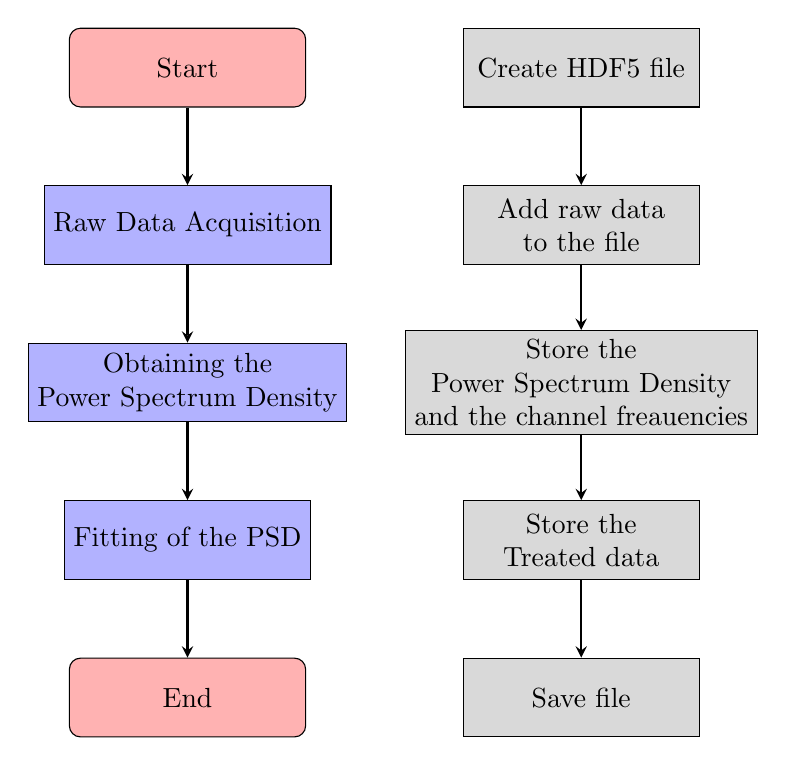
\begin{tikzpicture}[node distance=2cm]

        \node (start) [startstop] {Start};
        \node (acquire) [process, below of=start] {Raw Data Acquisition};
        \node (psd) [process, below of=acquire, align=center] {Obtaining the \\ Power Spectrum Density};
        \node (fits) [process, below of=psd] {Fitting of the PSD};
        \node (end) [startstop, below of=fits] {End};

        \draw [arrow] (start) -- (acquire);
        \draw [arrow] (acquire) -- (psd);
        \draw [arrow] (psd) -- (fits);
        \draw [arrow] (fits) -- (end);

        \node (filestart) [file, right of=start, xshift=3cm] {Create HDF5 file};
        \node (fileraw) [file, below of=filestart, align=center] {Add raw data \\ to the file};
        \node (filepsd) [file, below of=fileraw, align=center] {Store the \\ Power Spectrum Density\\and the channel freauencies};
        \node (filetreat) [file, below of=filepsd, align=center] {Store the \\ Treated data};
        \node (fileend) [file, below of=filetreat] {Save file};

        \draw [arrow] (filestart) -- (fileraw);
        \draw [arrow] (fileraw) -- (filepsd);
        \draw [arrow] (filepsd) -- (filetreat);
        \draw [arrow] (filetreat) -- (fileend);

        \end{tikzpicture}
        \end{center}

    % \subsection{Conceptual issues and envisionned solutions}
    
    %     \subsubsection{Raw Data Acquisition}
    %         Raw data will take a variety of form, and will sometimes need to be stored in combination with other data (e.g. array of time points). As such, we propose to store the raw data and all of the data it depends on for its understanding in the same group, naming "Raw Data" the array containing the measure of the energy of the signal, and "Abscissa\_i" all the other arrays that are used to understand the data. The resulting will therefore be the following:

    %         \begin{verbatim}
    %             file.h5
    %             +-- Data
    %             |   +-- Data_1
    %             |   |   +-- Raw_data
    %             |   |   +-- Abscissa_1
    %             |   |   +-- Abscissa_2
    %             |   |   +-- ...
    %             |   +-- ...
    %         \end{verbatim}

    %         It is imprecindible therefore to store the technique used to acquire the Brillouin spectrum in the attribute of the file. This information will be stored in the "SPECTROMETER.Type" attribute. 
    
    %     \subsubsection{Conversion of the data to a Power Spectrum Density}

    %         This is arguably the most important and controversial step of the pipeline. The goal of this step is to obtain the Power Spectrum Density of the data. Many different techniques can be used to do so, most of which will vary from laboratory to laboratory, and relying either on theoretical knowledge of the instrument or data calibration. As it is still unclear how to best convert the data to a PSD, we let the user choose the method they want to use. We propose to store the technique used in the "SPECTROMETER.PSD\_Method" attribute, following the following nomenclature: "Laboratory\_Method\_version". For example, the following attributes could be used:

    %         \begin{verbatim}
    %             SPECTROMETER.PSD_Method = "MedUniWien_1VIPA_1.0"
    %             SPECTROMETER.PSD_Method = "EMBL_2VIPA_0.5"
    %             SPECTROMETER.PSD_Method = "CellSense_CS363_2.5"
    %         \end{verbatim}

    %         Note that this conversion can be performed using an independent and even confidential pipeline, allowing firms to use this format without compromising their proprietary data. In the future, it might however be interesting to have a unified pipeline for all the techniques, which could automatically be adjusted to the "SPECTROMETER.Type" attribute. The end goal of this step is to obtain two arrays: 
    %         \begin{itemize}
    %             \item The "PSD" array, containing the PSD of the data.
    %             \item The "Channel\_frequencies" array, containing the channel frequencies of the data.
    %         \end{itemize}

    %         At this stage, the raw data might become irrelevant and costly in terms of storage space. We can therefore delete the "Raw\_data" array and the "Abscissa\_i" arrays associated to it at this stage. The resulting file would then take the following form:

    %         \begin{verbatim}
    %             file.h5
    %             +-- Data
    %             |   +-- Data_1
    %             |   |   +-- PSD
    %             |   |   +-- Frequency
    %             |   |   +-- ...
    %             |   +-- ...
    %         \end{verbatim}

    %         Alternatively, if different treatments are to be compared, we recommend creating different groups. The resulting file would then take the following form:

    %         \begin{verbatim}
    %             file.h5
    %             +-- Data
    %             |   +-- Data_1
    %             |   |   +-- Raw_data (optional)
    %             |   |   +-- Abscissa_1 (optional)
    %             |   |   +-- Data_1
    %             |   |   |   +-- PSD
    %             |   |   |   +-- Frequency
    %             |   |   +-- Data_2
    %             |   |   |   +-- PSD
    %             |   |   |   +-- Frequency
    %             |   |   +-- ...
    %             |   +-- ...
    %         \end{verbatim}

    %     \subsection{Fitting of the PSD}

    %         The fit of the Power Spectrum Density (PSD) can be unified in a single function that can accept parameters to precise the fit. We encourage you to refer to the dedicated notebook: \textbf{Treatment\_pipeline} found in the \textbf{guides} folder of the directory.

    %         The treatment should result in a new group "Treat\_i" composed of at least four arrays:
    %         \begin{itemize}
    %             \item The "Shift" array, containing the values of the fitted frequency shifts
    %             \item The "Linewidth" array, containing the values of the fitted linewidths
    %             \item The "Shift\_std" arrays, containing the variance of the fitted frequency shifts, used to auqntify the uncertainty of the fitted values
    %             \item The "Linewidth\_std" arrays, containing the variance of the fitted linewidths, used to auqntify the uncertainty of the fitted values
    %         \end{itemize}

    %         Additionnaly, other arrays can be added to the "Treat\_i" group, such as the "SNR" and "Amplitude" arrays, or any other relevant information extracted from the PSD.

    %         This treated group should in any case have as attributes all the parameters used in the treatment as well as the different steps followed for the treatment. 

    %         The returned structure should therefore be of the form:
    %         \begin{verbatim}
    %             file.h5
    %             +-- Data
    %             |   +-- Data_1
    %             |   |   +-- PSD
    %             |   |   +-- Frequency
    %             |   |   +-- Treat_1
    %             |   |   |   +-- Shift
    %             |   |   |   +-- Linewidth
    %             |   |   |   +-- Shift_std
    %             |   |   |   +-- Linewidth_std
    %             |   |   |   +-- ...
    %             |   +-- ...
    %         \end{verbatim}

    %         Other treatments on the same PSD can with this architecture be stored in the same file, by changing the index of the "Treat\_i" group. For example, if two peaks are to be fitted independently, the resulting file would take the following form:

    %         \begin{verbatim}
    %             file.h5
    %             +-- Data
    %             |   +-- Data_1
    %             |   |   +-- PSD
    %             |   |   +-- Frequency
    %             |   |   +-- Treat_1
    %             |   |   |   +-- Shift
    %             |   |   |   +-- Linewidth
    %             |   |   |   +-- Shift_std
    %             |   |   |   +-- Linewidth_std
    %             |   |   |   +-- ...
    %             |   |   +-- Treat_2
    %             |   |   |   +-- Shift
    %             |   |   |   +-- Linewidth
    %             |   |   |   +-- Shift_std
    %             |   |   |   +-- Linewidth_std
    %             |   |   |   +-- ...
    %             |   +-- ...
    %         \end{verbatim}


\end{document}